\documentclass[10pt,a4paper,spanish]{article}

\usepackage[spanish]{babel}
\usepackage[utf8]{inputenc}
\usepackage{amsmath, amsthm}
\usepackage{amsfonts, amssymb, latexsym}
\usepackage{enumerate}
% \usepackage[official]{eurosym}
\usepackage{graphicx}
\usepackage[usenames, dvipsnames]{color}
\usepackage{colortbl}
\usepackage{multirow}
\usepackage{fancyhdr}
\usepackage[all]{xy}
% \usepackage{minted}
\usepackage{float}
\usepackage{subfigure}
\usepackage{tikz}
\usepackage{pgfplots}
\usepackage{cancel}
\pgfplotsset{compat=1.5}

\usepackage[top=2.5cm, bottom=2.5cm, left=3cm, right=3cm]{geometry}

\usepackage[bookmarks=true,
            bookmarksnumbered=false, % true means bookmarks in
                                     % left window are numbered
            bookmarksopen=false,     % true means only level 1
                                     % are displayed.
            colorlinks=true,
            linkcolor=red,
            citecolor=blue]{hyperref}

\newcommand{\HRule}{\rule{\linewidth}{0.5mm}} % regla horizontal para  el titulo

\pagestyle{plain}
%con esto nos aseguramos de que las cabeceras de capítulo y de sección vayan en minúsculas

\fancyhf{} %borra cabecera y pie actuales
% \fancyhead[LE,RO]{}
% \fancyhead[LO]{}
\fancyfoot[C]{\thepage}
% \renewcommand{\headrulewidth}{0.5pt}
% \renewcommand{\footrulewidth}{0pt}
% \addtolength{\headheight}{0.5pt} %espacio para la raya
% \fancypagestyle{plain}{%
%       \fancyhead{} %elimina cabeceras en páginas "plain"
%       \renewcommand{\headrulewidth}{0pt} %así como la raya
% }

% %%%%% Para cambiar el tipo de letra en el título de la sección %%%%%%%%%%%
% \usepackage{sectsty}
% \chapterfont{\fontfamily{frc}\selectfont}
% \sectionfont{\fontfamily{pag}\selectfont}
% \subsectionfont{\fontfamily{pag}\selectfont}
% \subsubsectionfont{\fontfamily{pag}\selectfont}

% \newmintedfile[mycplusplus]{c++}{
%     linenos,
%     numbersep=5pt,
%     gobble=0,
%     frame=lines,
%     framesep=2mm,
%     tabsize=3,
% }

% \newmintedfile[mypython]{python}{
%     linenos,
%     numbersep=5pt,
%     gobble=0,
%     frame=lines,
%     framesep=2mm,
%     tabsize=3,
% }

\definecolor{amaranth}{rgb}{0.9, 0.17, 0.31}

\usepackage{arev}
\usepackage[T1]{fontenc}

\setlength{\parindent}{0pt}
\setlength{\parskip}{1ex plus 0.5ex minus 0.2ex}

% \usepackage{titlesec}

% % \titleformat{\chapter}{\normalfont\huge\center}{--- \thechapter ---}{20pt}{}

% \titleformat
% {\chapter} % command
% [display] % shape
% {\Huge\center\bfseries} % format
% {--- \thechapter ---} % label
% {0.5ex} % sep
% {
%     \rule{\textwidth}{1pt}
%     \vspace{1ex}
%     \centering
% } % before-code
% [
% \vspace{-0.5ex}%
% \rule{\textwidth}{0.3pt}
% ] % after-code

%Definimos autor y título
\title{\Huge Arquitectura de las Redes \textit{Tor}}
\author{\Large Marta Gómez Macías y Braulio Vargas López}

\begin{document}
\renewcommand{\tablename}{Tabla}
\maketitle

\tableofcontents

\section{¿Qué es \textit{Tor}?}
Según \cite{deftor}, ``la red Tor es un grupo de servidores operativos voluntarios que permiten a las personas mejorar su privacidad y seguridad en Internet''. Esto quiere decir que una conexión a través de Tor nunca será directa, sino que pasará por estos servidores voluntarios para que no se pueda saber quién manda el paquete ni a dónde va dirigido. Además, Tor también se define como ``una efectiva herramienta para la elusión de la censura, permitiendo a sus usuarios acceder a contenido que de otra forma se encontraría bloqueado.''

\subsection{¿Por qué es \textit{Tor} protege mejor la privacidad que otras herramientas?}
Tal y como se explica en \cite{deftor}, usando Tor nos protegemos contra el ``análisis de tráfico''. Aunque el \textit{payload} de los paquetes que enviamos a través de la red se encuentre encriptado, la cabecera normalmente no suele estarlo ya que se necesita para dirigir el paquete. Ésta cabecera facilita a los ``sniffers'' muchísima información sobre lo que estamos haciendo ya que incluye información como el ``host'' emisor, el ``host'' destino, el tamaño, el puerto al que va dirigido, etc.

Así, tal y como se indica en \cite{protectionstor}, Tor defiende la privacidad en tres sentidos:
\begin{enumerate}[$\bullet$]
    \item Evita que servicios tales como páginas webs (entre otros) sepan nuestra localización, la cual pueden usar para hacer una base de datos sobre nuestras costumbres e intereses. Con \textit{Tor} podemos elegir qué información compartimos y cuál no.
    \item Evita el análisis de nuestro tráfico (que, por ejemplo, puede hacer nuestro proveedor de internet) viendo la información que compartimos y desde dónde. Y también nos permite acceder a sitios web bloqueados.
    \item Tor dirige nuestra conexión por más de un \textit{relay}\footnote{Un \textit{relay} se refiere a cada servidor por el cual se envían nuestros paquetes.}, por lo que ningún \textit{relay} puede saber lo que hacemos. Esta arquitectura de \textit{relays} distribuidos (y que pertenecen a distintas personas/organizaciones) da mayor privacidad.
\end{enumerate}

Ahora bien, tal y como se aclara en \cite{anonymoustor}, usar Tor no es sinónimo de ser completamente anónimo en internet, pues lo único que protege Tor es la ruta de los paquetes que enviamos y no su contenido. Por lo que si, por ejemplo, nos conectamos a \textit{Facebook} desde Tor, \textit{Facebook} no sabrá desde dónde nos estamos conectando pero sí que sabrá nuestra identidad.

\section{Arquitectura de Tor}

El anonimato en \textit{Tor} se mantiene distribuyendo los paquetes que enviamos y recibimos por una gran cantidad de puntos distribuidos por internet, antes de llegar al destino, en vez de hacer una conexión directa entre el origen y el destino. Los paquetes de datos seguirán un camino aleatorio entre los distintos ``relevos'' que existen en la red de Tor, que eliminan nuestras $huellas$, para que en ningún punto del camino que toma el paquete se pueda saber de dónde viene el paquete y a dónde va.

Para crear un camino en la red privada de Tor, se crea un circuito incremental de conexiones encriptadas a través de los ``relevos'' de la red, como podemos ver en la \hyperref[htw1]{Figura \ref*{htw1}}. Los incrementos del circuito se hacen de uno en uno cada vez, y cada punto del circuito sólo sabe de qué relevo viene el paquete, y a qué relevo se lo tiene que dar. El cliente aporta un conjunto de llaves diferentes para encriptar el mensaje para cada punto del circuito para asegurarse de que en cada punto del circuito no se pueda seguir el paquete (\hyperref[htw2]{Figura \ref*{htw2}}). Gracias a esto, como un nodo solo conoce de qué nodo viene la información y a qué nodo tiene que mandarla, 

Por eficiencia, el mismo circuito tiene una vida de 10 minutos más o menos. Para las siguientes conexiones obtienen un nuevo circuito, como se ve en la \hyperref[htw3]{Figura \ref*{htw3}}.

\begin{figure}[H]
    \centering
    
    \mbox {
        \subfigure[Inicio de la conexión Tor. Al inicio de la conexión obtenemos una lista de nodos Tor del directorio del servidor.]{
            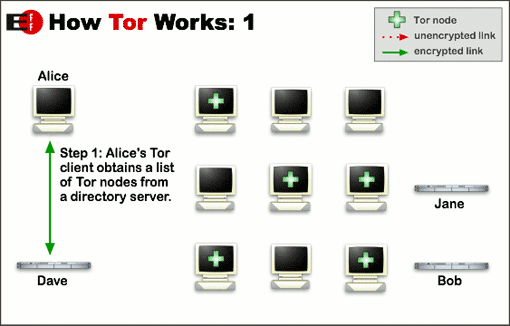
\includegraphics[width=0.5\textwidth]{htw1}
            \label{htw1}
        }
        
        \qquad
    
        \subfigure[Circuito o camino creado para la conexión. Como se ve en la imagen, los enlaces en verde están encriptados y los rojos no.] {
            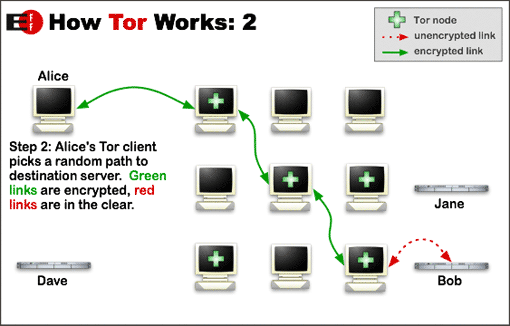
\includegraphics[width=0.51\textwidth]{htw2}
            \label{htw2}
        }
    }

    \mbox{
        \subfigure[Si se realiza una conexión más allá de esos 10 minutos, se genera un nuevo circuito.] {
            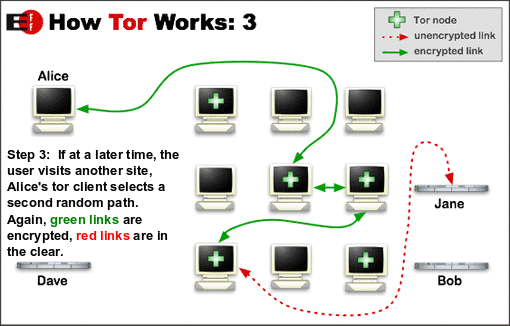
\includegraphics[width=0.51\textwidth]{htw3}
            \label{htw3}
        }
    }
    \caption{Cómo funciona Tor.}
    \label{htw}
\end{figure} 

\section{Protocolo}
El protocolo de Tor se basa en una serie de protocolos seguros y parámetros de seguridad para la comunicación y envío de información, como se ve en \cite{torproc}. Es decir, es un protocolo \textit{End-to-End encryption}, en el que los datos se encriptan para poder enviarlos a través de un canal vulnerable, hasta que llegan al destinatario, donde puede ser desencriptado.

Para ello utiliza lo siguiente:

\begin{description}
    \item [Cifrado de \textit{stream}:] En este caso, cifra el \textit{stream} de datos mediante el algoritmo $AES-128~bits$
    \item [Cifrado de llave pública:] Para ello, utiliza claves $RSA$ con 1024-$bits$ (y un exponente fijo de 65537).
    \item [Protocolo Diffie-Hellman:] consiste en un protocolo criptográfico para establecer claves entre dos partes que no han tenido contacto previo, a través de un canal inseguro y anónimamente. Este protocolo consiste en coger un número primo al azar conococido, es decir público, y un número perteneciente al anillo formado por el primo inferior que será privado. Entonces, ambas partes hacen operaciones matemáticas con estos números que incluyen la exponenciación y se envían los resultados. Ambas partes, con los números que disponen son capaces de llegar a la misma solución o clave.
    \item [Función Hash:] se usa para hacer el digest de los datos. Para ello utiliza el algoritmo SHA-1.
\end{description}

El tráfico que fluye a través del circuito, se envía en celdas de tamaño fijo, envueltas por una clave simétrica en cada nodo y enviada al siguiente nodo del circuito. 

\subsubsection{¿Cómo se realiza la conexión entre los nodos?}

La conexión entre dos nodos, o entre un cliente y un nodo, se realiza usando una conexión \textit{TLS/SSLv3} para la identificación de los enlaces y la encriptación del tráfico. Para la realización del ``\textit{handshake}'' entre los nodos, existen tres maneras diferentes de hacerlo:

\begin{enumerate}
    \item \textbf{``\textit{Certificates-up-front}'' o ``\textit{the v1 handshake}''}: el que inicia la conexión y el que responde se intercambian una cadena de certifcados como parte de su $handshake$. El que inicia la conexión envía dos certificados. En el primer certificado, envía una clave pública de corta duración y en el segundo se envía su clave identificadora.

    \item \textbf{``\textit{Renegotiation}'' o ``\textit{the v2 handshake}''}: en este caso sólo se envía un único certificado por parte del que responde la solicitud de conexión y el solicitante realiza la conexión, inicia una renegociación $TLS$\footnote{esto consiste en volver a repetir la ``negociación'' del intercambio de claves.}. A partir de aquí, se realizan el mismo intercambio que en la versión 1.

    \item \textbf{``\textit{In-protocol}'' o ``\textit{the v3 handshake}''}: el que inicia la conexión no envía ningún certificado, y el que responde envía un único certificado. Entonces se escogerá una \textit{ciphersuite} entre el cliente y el servidor, en la que vendrá indicado el algoritmo para el establecimiento de la clave, el algoritmo de autenticación de la clave y los algoritmos para hacer el digest, como se puede ver en \cite{ciphersuite}.
\end{enumerate}

En ninguno de los handshakes anteriores se debe contener información que pueda identificar al host o al nodo. A la hora de realizar una renegociación, las ciphersuites se eligen aquellas ciphersuites y extensiones TLS que puedan mimetizar aquellas que puedan ser usadas por un navegador popular.

Una vez realizado el handshake y se han intercambiado lo scertificados, se debe comprobar que la identity key es la esperada, tanto durante el inicio de la conexión, que la aporta el certificado, o durante la conexión que viene en el paquete. Si esta clave no es la real, se cierra inmediatamente la conexión.

Una vez que la conexión TLS ha sido establecida, ambas partes se envían los paquetes de forma secuencial, protegidos por la conexión TLS y los correspondientes cifrados de los nodos.

Una vez explicado esto, vamos a ver un ejemplo de conexión, usando la \hyperref[comunicaciones]{Figura \ref*{comunicaciones}}. En ella podemos ver como el usuario quiere realizar una conexión con un website.

Para ello, se realizan varios pasos:
\begin{enumerate}
    \item Lo primero que hará el cliente será descargarse la lista de nodos Tor de un servidor que almacena este directorio.
    \item Tras esto, coge un primer nodo (o relay) al azar para comenzar a construir el circuito. A través de un tunel TLS, realiza el $handshake$ con el servidor y el intercambio de claves con el protocolo Diffie-Hellman, y establecen la clave. Tras esto, el cliente vuelve a realizar una extensión del circuito, siendo el primer relay del circuito quien realiza la conexión. De esta forma, el segundo relay sólo conoce al primer relay, sin saber nada del cliente. Al establecer el $handshake$ con el pirmer relay, el cliente también obtiene la clave para el cifrado entre el primer y segundo relay. En este caso, se da por finalizada la construcción del circuito.
    \item A continuación, el cliente solicita una conexión a un $website$ en el puerto 80. Esta solicitud es cifrada por el propio cliente con la clave del primer relay, y con la clave del segundo, creando unas capas criptográficas, simulando las capas de una cebolla, como las que se pueden ver en la \hyperref[cebollas]{Figura \ref*{cebollas}} y se le envía al primer relay.
    
    \begin{figure}[!h]
        \centering
        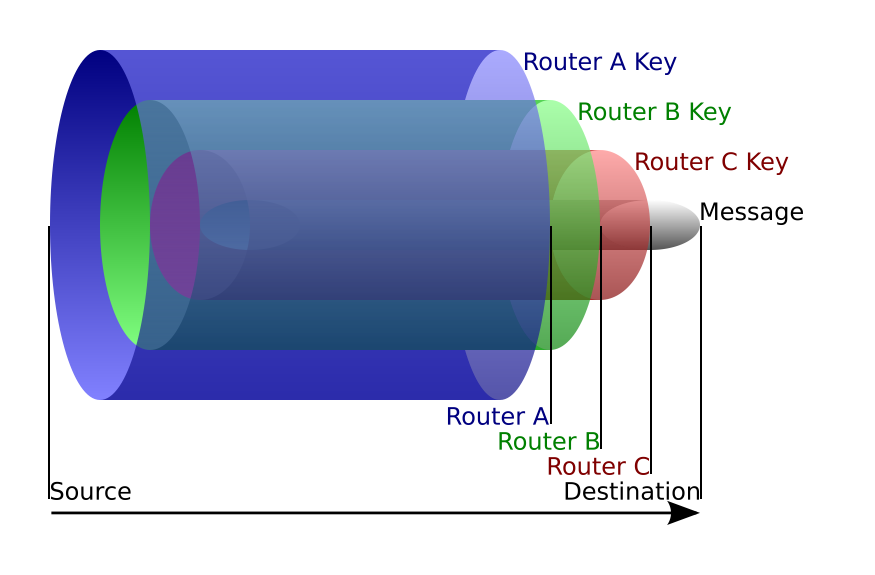
\includegraphics[width=0.6\textwidth]{Onion}
        \caption{\textit{Onion diagram}, según \cite{cebollas}.}
        \label{cebollas}
    \end{figure}

    \item Una vez en el primer relay, se descifra la primera capa del cifrado con su clave y se le envía al segundo relay, el cual quitará la capa que queda y pasará el mensaje sin cifrar al website. Este es el único momento en el que los datos no estarán cifrados, como se ve en la \hyperref[htw2]{Figura \ref*{htw2}}.

    \item Tras esto, el servidor responde la petición del segundo relay y este obtiene los datos del $website$. Después, los cifra con su clave y se los pasa al relay anterior, comenzando a crear las capas otra vez.

    \item Al llegar al primer relay, este se vuelve a cifrar con su clave y se le pasa al cliente, que al tener todas las claves, es capaz de descifrar el mensaje y obtener los datos del $website$.

\end{enumerate}

\subsection{Estructura de un paquete}
En la sección ``The Tor Design'' de \cite{design}, encontramos una descripción detallada de la arquitectura de \textit{Tor}. Un paquete Tor tiene exactamente 512 bytes y está compuesto por una cabecera y un payload. 

En la \hyperref[paquete]{Figura \ref*{paquete}} vemos una representación gráfica de un paquete Tor. La cabecera incluye tanto el identificador del circuito (que indica a qué circuito pertenece el paquete) como un comando que describe qué hacer con el payload. Según sea dicho comando, los paquetes pueden ser tanto de \textbf{control} como de \textbf{relay}. Un paquete de control debe ser interpretado por el nodo que lo recibe y sirve para operar con el circuito y uno de relay, sólo contiene datos.

Los paquetes \textit{relay} tienen una cabecera adicional antes del payload. Ésta cabecera contiene el \textit{streamID}, un \textit{checksum} para poder hacer una comprobación de integridad, la longitud del payload y un comando \textit{relay}, que puede tomar valores para operar tanto con el stream de datos como con el circuito y para hacer un control de congestión.

\begin{figure}[!h]
    \centering
    % Graphic for TeX using PGF
% Title: /home/marta/Documentos/Git/Arquitectura-Redes-Tor/PDFResumen/Diagrama1.dia
% Creator: Dia v0.97.3
% CreationDate: Tue Dec  8 21:22:44 2015
% For: marta
% \usepackage{tikz}
% The following commands are not supported in PSTricks at present
% We define them conditionally, so when they are implemented,
% this pgf file will use them.
\ifx\du\undefined
  \newlength{\du}
\fi
\setlength{\du}{15\unitlength}
\begin{tikzpicture}
\pgftransformxscale{1.000000}
\pgftransformyscale{-1.000000}
\definecolor{dialinecolor}{rgb}{0.000000, 0.000000, 0.000000}
\pgfsetstrokecolor{dialinecolor}
\definecolor{dialinecolor}{rgb}{1.000000, 1.000000, 1.000000}
\pgfsetfillcolor{dialinecolor}
\definecolor{dialinecolor}{rgb}{1.000000, 1.000000, 1.000000}
\pgfsetfillcolor{dialinecolor}
\fill (5.100000\du,5.000000\du)--(5.100000\du,6.900000\du)--(10.050000\du,6.900000\du)--(10.050000\du,5.000000\du)--cycle;
\pgfsetlinewidth{0.100000\du}
\pgfsetdash{}{0pt}
\pgfsetdash{}{0pt}
\pgfsetmiterjoin
\definecolor{dialinecolor}{rgb}{0.000000, 0.000000, 0.000000}
\pgfsetstrokecolor{dialinecolor}
\draw (5.100000\du,5.000000\du)--(5.100000\du,6.900000\du)--(10.050000\du,6.900000\du)--(10.050000\du,5.000000\du)--cycle;
% setfont left to latex
\definecolor{dialinecolor}{rgb}{0.000000, 0.000000, 0.000000}
\pgfsetstrokecolor{dialinecolor}
\node at (7.575000\du,6.145000\du){CircID};
% setfont left to latex
\definecolor{dialinecolor}{rgb}{0.000000, 0.000000, 0.000000}
\pgfsetstrokecolor{dialinecolor}
\node[anchor=west] at (7.450000\du,4.500000\du){2};
\definecolor{dialinecolor}{rgb}{1.000000, 1.000000, 1.000000}
\pgfsetfillcolor{dialinecolor}
\fill (10.053750\du,5.000000\du)--(10.053750\du,6.900000\du)--(12.646250\du,6.900000\du)--(12.646250\du,5.000000\du)--cycle;
\pgfsetlinewidth{0.100000\du}
\pgfsetdash{}{0pt}
\pgfsetdash{}{0pt}
\pgfsetmiterjoin
\definecolor{dialinecolor}{rgb}{0.000000, 0.000000, 0.000000}
\pgfsetstrokecolor{dialinecolor}
\draw (10.053750\du,5.000000\du)--(10.053750\du,6.900000\du)--(12.646250\du,6.900000\du)--(12.646250\du,5.000000\du)--cycle;
% setfont left to latex
\definecolor{dialinecolor}{rgb}{0.000000, 0.000000, 0.000000}
\pgfsetstrokecolor{dialinecolor}
\node at (11.350000\du,6.145000\du){CMD};
% setfont left to latex
\definecolor{dialinecolor}{rgb}{0.000000, 0.000000, 0.000000}
\pgfsetstrokecolor{dialinecolor}
\node[anchor=west] at (11.300000\du,4.350000\du){1};
\definecolor{dialinecolor}{rgb}{1.000000, 1.000000, 1.000000}
\pgfsetfillcolor{dialinecolor}
\fill (12.700000\du,5.000000\du)--(12.700000\du,6.900000\du)--(26.950000\du,6.900000\du)--(26.950000\du,5.000000\du)--cycle;
\pgfsetlinewidth{0.100000\du}
\pgfsetdash{}{0pt}
\pgfsetdash{}{0pt}
\pgfsetmiterjoin
\definecolor{dialinecolor}{rgb}{0.000000, 0.000000, 0.000000}
\pgfsetstrokecolor{dialinecolor}
\draw (12.700000\du,5.000000\du)--(12.700000\du,6.900000\du)--(26.950000\du,6.900000\du)--(26.950000\du,5.000000\du)--cycle;
% setfont left to latex
\definecolor{dialinecolor}{rgb}{0.000000, 0.000000, 0.000000}
\pgfsetstrokecolor{dialinecolor}
\node at (19.825000\du,6.145000\du){DATA};
% setfont left to latex
\definecolor{dialinecolor}{rgb}{0.000000, 0.000000, 0.000000}
\pgfsetstrokecolor{dialinecolor}
\node[anchor=west] at (18.100000\du,4.600000\du){509  bytes};
\definecolor{dialinecolor}{rgb}{1.000000, 1.000000, 1.000000}
\pgfsetfillcolor{dialinecolor}
\fill (4.996250\du,8.100000\du)--(4.996250\du,10.000000\du)--(8.003750\du,10.000000\du)--(8.003750\du,8.100000\du)--cycle;
\pgfsetlinewidth{0.100000\du}
\pgfsetdash{}{0pt}
\pgfsetdash{}{0pt}
\pgfsetmiterjoin
\definecolor{dialinecolor}{rgb}{0.000000, 0.000000, 0.000000}
\pgfsetstrokecolor{dialinecolor}
\draw (4.996250\du,8.100000\du)--(4.996250\du,10.000000\du)--(8.003750\du,10.000000\du)--(8.003750\du,8.100000\du)--cycle;
% setfont left to latex
\definecolor{dialinecolor}{rgb}{0.000000, 0.000000, 0.000000}
\pgfsetstrokecolor{dialinecolor}
\node at (6.500000\du,9.245000\du){CircID};
% setfont left to latex
\definecolor{dialinecolor}{rgb}{0.000000, 0.000000, 0.000000}
\pgfsetstrokecolor{dialinecolor}
\node[anchor=west] at (6.363388\du,7.712500\du){2};
\definecolor{dialinecolor}{rgb}{1.000000, 1.000000, 1.000000}
\pgfsetfillcolor{dialinecolor}
\fill (7.968750\du,8.100000\du)--(7.968750\du,10.000000\du)--(10.831250\du,10.000000\du)--(10.831250\du,8.100000\du)--cycle;
\pgfsetlinewidth{0.100000\du}
\pgfsetdash{}{0pt}
\pgfsetdash{}{0pt}
\pgfsetmiterjoin
\definecolor{dialinecolor}{rgb}{0.000000, 0.000000, 0.000000}
\pgfsetstrokecolor{dialinecolor}
\draw (7.968750\du,8.100000\du)--(7.968750\du,10.000000\du)--(10.831250\du,10.000000\du)--(10.831250\du,8.100000\du)--cycle;
% setfont left to latex
\definecolor{dialinecolor}{rgb}{0.000000, 0.000000, 0.000000}
\pgfsetstrokecolor{dialinecolor}
\node at (9.400000\du,9.245000\du){Relay};
% setfont left to latex
\definecolor{dialinecolor}{rgb}{0.000000, 0.000000, 0.000000}
\pgfsetstrokecolor{dialinecolor}
\node[anchor=west] at (9.313020\du,7.688388\du){1};
\definecolor{dialinecolor}{rgb}{1.000000, 1.000000, 1.000000}
\pgfsetfillcolor{dialinecolor}
\fill (10.801250\du,8.100000\du)--(10.801250\du,10.000000\du)--(14.898750\du,10.000000\du)--(14.898750\du,8.100000\du)--cycle;
\pgfsetlinewidth{0.100000\du}
\pgfsetdash{}{0pt}
\pgfsetdash{}{0pt}
\pgfsetmiterjoin
\definecolor{dialinecolor}{rgb}{0.000000, 0.000000, 0.000000}
\pgfsetstrokecolor{dialinecolor}
\draw (10.801250\du,8.100000\du)--(10.801250\du,10.000000\du)--(14.898750\du,10.000000\du)--(14.898750\du,8.100000\du)--cycle;
% setfont left to latex
\definecolor{dialinecolor}{rgb}{0.000000, 0.000000, 0.000000}
\pgfsetstrokecolor{dialinecolor}
\node at (12.850000\du,9.245000\du){StreamID};
% setfont left to latex
\definecolor{dialinecolor}{rgb}{0.000000, 0.000000, 0.000000}
\pgfsetstrokecolor{dialinecolor}
\node[anchor=west] at (12.557322\du,7.658211\du){2};
\definecolor{dialinecolor}{rgb}{1.000000, 1.000000, 1.000000}
\pgfsetfillcolor{dialinecolor}
\fill (14.922500\du,8.100000\du)--(14.922500\du,10.000000\du)--(18.077500\du,10.000000\du)--(18.077500\du,8.100000\du)--cycle;
\pgfsetlinewidth{0.100000\du}
\pgfsetdash{}{0pt}
\pgfsetdash{}{0pt}
\pgfsetmiterjoin
\definecolor{dialinecolor}{rgb}{0.000000, 0.000000, 0.000000}
\pgfsetstrokecolor{dialinecolor}
\draw (14.922500\du,8.100000\du)--(14.922500\du,10.000000\du)--(18.077500\du,10.000000\du)--(18.077500\du,8.100000\du)--cycle;
% setfont left to latex
\definecolor{dialinecolor}{rgb}{0.000000, 0.000000, 0.000000}
\pgfsetstrokecolor{dialinecolor}
\node at (16.500000\du,9.245000\du){Digest};
% setfont left to latex
\definecolor{dialinecolor}{rgb}{0.000000, 0.000000, 0.000000}
\pgfsetstrokecolor{dialinecolor}
\node[anchor=west] at (16.337500\du,7.700000\du){6};
\definecolor{dialinecolor}{rgb}{1.000000, 1.000000, 1.000000}
\pgfsetfillcolor{dialinecolor}
\fill (18.026250\du,8.100000\du)--(18.026250\du,10.000000\du)--(20.273750\du,10.000000\du)--(20.273750\du,8.100000\du)--cycle;
\pgfsetlinewidth{0.100000\du}
\pgfsetdash{}{0pt}
\pgfsetdash{}{0pt}
\pgfsetmiterjoin
\definecolor{dialinecolor}{rgb}{0.000000, 0.000000, 0.000000}
\pgfsetstrokecolor{dialinecolor}
\draw (18.026250\du,8.100000\du)--(18.026250\du,10.000000\du)--(20.273750\du,10.000000\du)--(20.273750\du,8.100000\du)--cycle;
% setfont left to latex
\definecolor{dialinecolor}{rgb}{0.000000, 0.000000, 0.000000}
\pgfsetstrokecolor{dialinecolor}
\node at (19.150000\du,9.245000\du){Len};
% setfont left to latex
\definecolor{dialinecolor}{rgb}{0.000000, 0.000000, 0.000000}
\pgfsetstrokecolor{dialinecolor}
\node[anchor=west] at (18.937500\du,7.675000\du){2};
\definecolor{dialinecolor}{rgb}{1.000000, 1.000000, 1.000000}
\pgfsetfillcolor{dialinecolor}
\fill (20.225000\du,8.100000\du)--(20.225000\du,10.000000\du)--(22.817500\du,10.000000\du)--(22.817500\du,8.100000\du)--cycle;
\pgfsetlinewidth{0.100000\du}
\pgfsetdash{}{0pt}
\pgfsetdash{}{0pt}
\pgfsetmiterjoin
\definecolor{dialinecolor}{rgb}{0.000000, 0.000000, 0.000000}
\pgfsetstrokecolor{dialinecolor}
\draw (20.225000\du,8.100000\du)--(20.225000\du,10.000000\du)--(22.817500\du,10.000000\du)--(22.817500\du,8.100000\du)--cycle;
% setfont left to latex
\definecolor{dialinecolor}{rgb}{0.000000, 0.000000, 0.000000}
\pgfsetstrokecolor{dialinecolor}
\node at (21.521250\du,9.245000\du){CMD};
% setfont left to latex
\definecolor{dialinecolor}{rgb}{0.000000, 0.000000, 0.000000}
\pgfsetstrokecolor{dialinecolor}
\node[anchor=west] at (21.312500\du,7.700000\du){1};
\definecolor{dialinecolor}{rgb}{1.000000, 1.000000, 1.000000}
\pgfsetfillcolor{dialinecolor}
\fill (22.776250\du,8.100000\du)--(22.776250\du,10.000000\du)--(27.050000\du,10.000000\du)--(27.050000\du,8.100000\du)--cycle;
\pgfsetlinewidth{0.100000\du}
\pgfsetdash{}{0pt}
\pgfsetdash{}{0pt}
\pgfsetmiterjoin
\definecolor{dialinecolor}{rgb}{0.000000, 0.000000, 0.000000}
\pgfsetstrokecolor{dialinecolor}
\draw (22.776250\du,8.100000\du)--(22.776250\du,10.000000\du)--(27.050000\du,10.000000\du)--(27.050000\du,8.100000\du)--cycle;
% setfont left to latex
\definecolor{dialinecolor}{rgb}{0.000000, 0.000000, 0.000000}
\pgfsetstrokecolor{dialinecolor}
\node at (24.913125\du,9.245000\du){DATA};
% setfont left to latex
\definecolor{dialinecolor}{rgb}{0.000000, 0.000000, 0.000000}
\pgfsetstrokecolor{dialinecolor}
\node[anchor=west] at (24.550000\du,7.675000\du){498};
\end{tikzpicture}

    \caption{Arquitectura de un paquete Tor}
    \label{paquete}
\end{figure}

Los dos tipos de cabeceras estudiados se encriptan y desencriptan en cada nodo del circuito usando el algoritmo de encriptación AES con 128-bits.
\begin{figure}[!h]
    \centering
    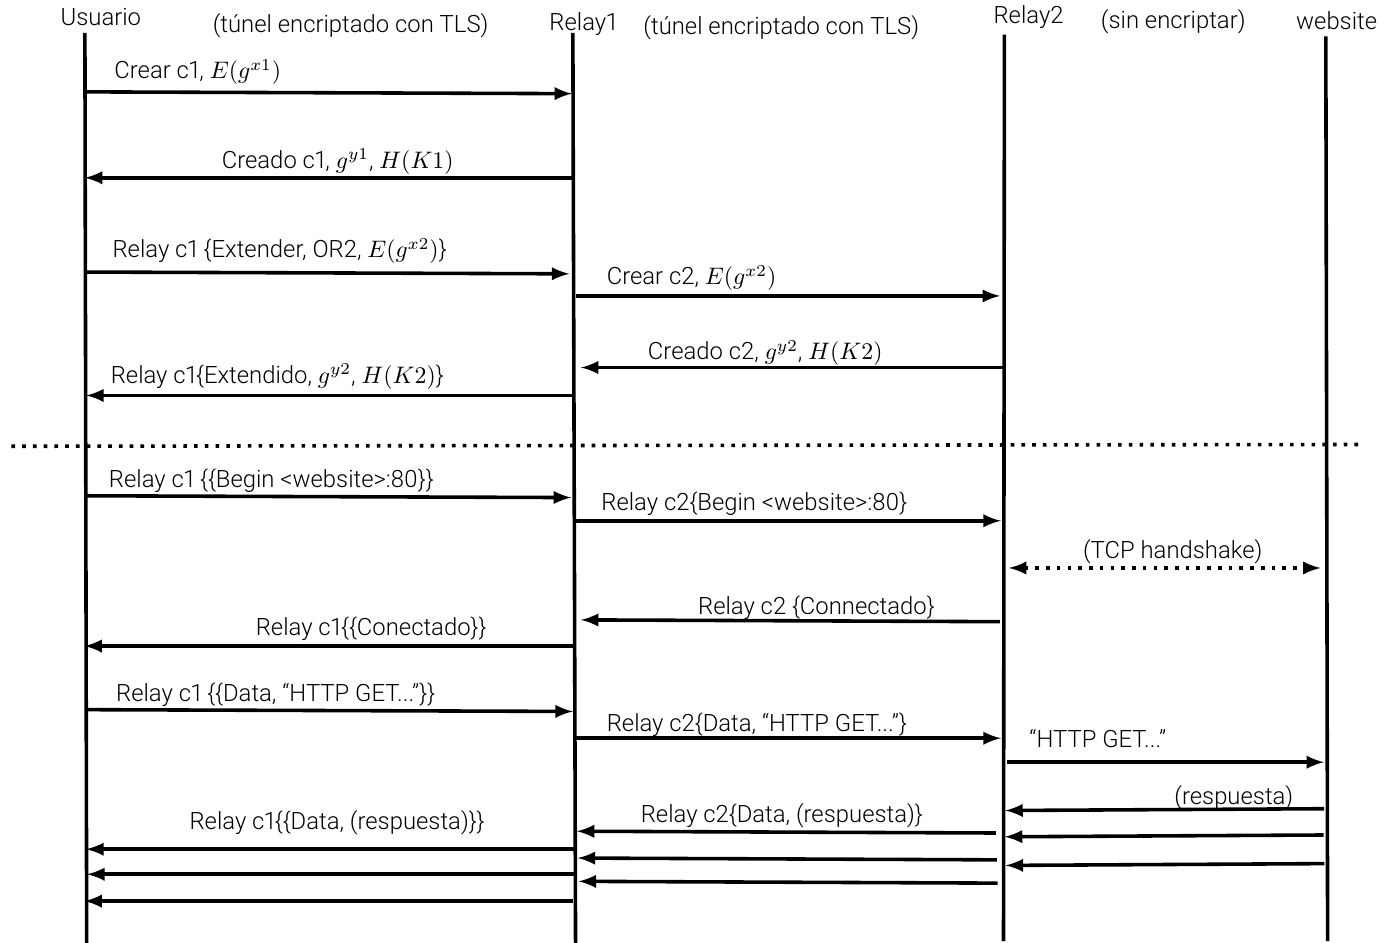
\includegraphics[width=1\textwidth]{comunicaciones}
    \caption{Ejemplo de una conexión usando Tor.}
    \label{comunicaciones}
\end{figure}

\section{Servicios ocultos}
En \cite{hiddenservices} encontramos una explicación acerca de los \textbf{servicios ocultos} en Tor. Un \textit{servicio oculto} es un servicio, como por ejemplo una página web o un servicio de mensajería instantánea, que funciona sin tener una dirección IP pública. Para ello, se usan los \textit{rendezvous points} de Tor.

En primer lugar, un servicio oculto debe advertir de su presencia en la red Tor. Para ello, tal y como se ve en la \hyperref[ths1]{Figura \ref*{ths1}}, escoge aleatoriamente unos cuantos relays, construye circuitos (no conexiones directas) hacia ellos y les pide actuar como \textit{introduction points} proporcionándoles su clave pública. Gracias a que usamos un circuito Tor y no una conexión directa, no se podrá asociar un \textit{introduction point} con la dirección IP del servicio oculto.

\begin{figure}[!h]
    \centering
    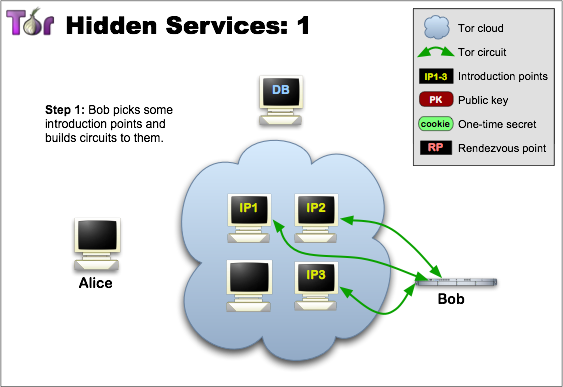
\includegraphics[width=0.5\textwidth]{THS-1}
    \caption{El servicio oculto, a través de circuitos Tor, da su clave pública a los relays que aleatoriamente ha escogido como \textit{introduction points}}
    \label{ths1}
\end{figure}

Tras esto, como se ve en la \hyperref[ths2]{Figura \ref*{ths2}}, el servicio oculto construye un \textit{descriptor de servicio oculto}, que contiene su clave pública y un resumen de cada punto de introducción y lo firma con su clave privada. Cuando los clientes pidan la dirección \texttt{XYZ.onion}, donde \textit{XYZ} es un nombre con 16 caracteres derivado de la clave pública del servidor, accederán al descriptor de servicio oculto. El hecho de que el nombre del servicio sea generado automáticamente por un derivado de su clave pública asegura a todo el que se comunique con él que están hablando con el servicio correcto. Es decir, sirve como verificación.

\begin{figure}[!h]
    \centering
    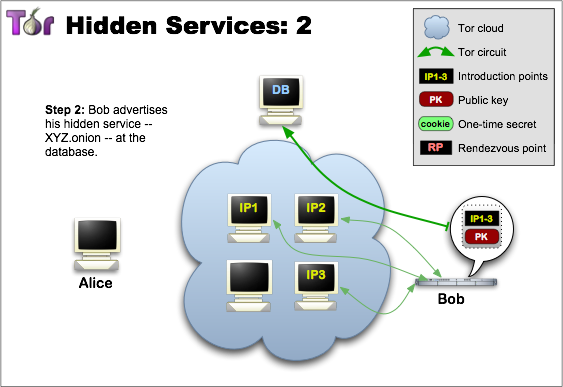
\includegraphics[width=0.5\textwidth]{THS-2}
    \caption{El servicio oculto, construye su descriptor de servicio oculto y lo sube a la base de datos.}
    \label{ths2}
\end{figure}

Cuando un cliente quiere conectarse a un servicio oculto concreto necesita saber su dirección \texttt{XYZ.onion}. Una vez sabida, descarga de la tabla hash el descriptor del servicio para saber la clave pública y el conjunto de puntos de introducción. También debe escoger un relay aleatoriamente para pedirle que actue como punto \textit{rendezvous} contándole un secreto ``one-time'' (\hyperref[ths3]{Figura \ref*{ths3}}).

\begin{figure}[!h]
    \centering
    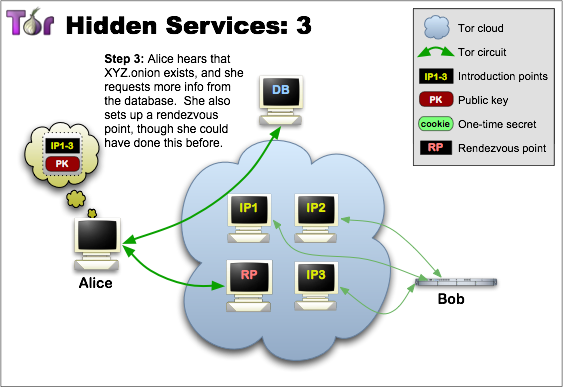
\includegraphics[width=0.5\textwidth]{THS-3}
    \caption{Cuando el cliente quiere conectarse, descarga el descriptor correspondiente a XYZ.onion de la base de datos y establece un punto de quedada.}
    \label{ths3}
\end{figure}

Una vez preparados el punto \textit{rendezvous} y el descriptor, tal y como se aprecia en la \hyperref[ths4]{Figura \ref*{ths4}} el cliente ensambla un mensaje de introducción encriptado con la clave pública del servidor que incluye el punto \textit{rendezvous} y el secreto ``one-time'' y lo envía a los puntos de introducción, pidiéndoles que lo envíen al servicio oculto. Como todo ésto se hace a través de una red Tor, es imposible relacionar la identidad del cliente con el mensaje de introducción.

\begin{figure}[!h]
    \centering
    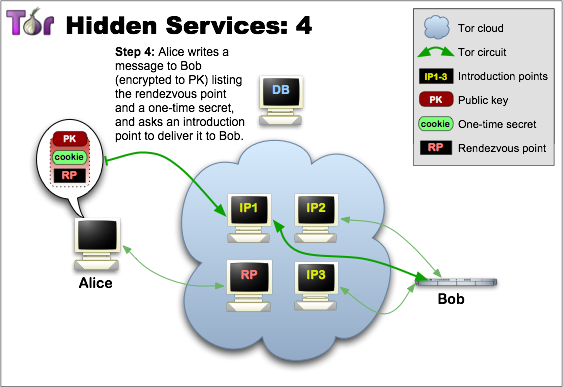
\includegraphics[width=0.5\textwidth]{THS-4}
    \caption{El cliente le comunica al servicio oculto el punto de quedada y el secreto ``one-time''}
    \label{ths4}
\end{figure}

El servicio oculto desencripta el mensaje de introducción del cliente y encuentra así tanto la dirección del punto \textit{rendezvous} como el secreto ``one-time''. Entonces, crea un circuito hacia el punto \textit{rendezvous} y le envía el secreto ``one-time'' (\hyperref[ths5]{Figura \ref*{ths5}}). Es muy importante que el servicio oculto se atenga al mismo conjunto de \textit{guardias de entrada}\footnote{Según \cite{entryguards}, los guardias de entrada se usan para evitar que un atacante controle o pueda sacar información controlando relays. Los usuarios seleccionan unos pocos relays al azar y son siempre los primeros que usan al acceder a la red Tor.} a la hora de crear nuevos circuitos ya que si no un atacante podría obtener la IP del servicio oculto obligándolo a crear nuevos circuitos y esperando a que el servicio oculto escoja el relay controlado por él.

\begin{figure}[!h]
    \centering
    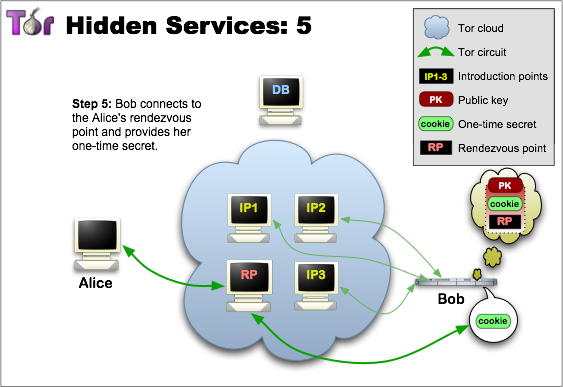
\includegraphics[width=0.5\textwidth]{THS-5}
    \caption{El servicio oculto desencripta el mensaje de introducción y se conecta al punto de quedada usando el secreto ``one-time'' que ha establecido el cliente.}
    \label{ths5}
\end{figure}

Por último, el punto \textit{rendezvous} notifica al cliente de que la conexión con el servidor ha ido bien y ambos empiezan a comunicarse usando los circuitos que habían hecho hacia el punto \textit{rendezvous}, que acúa como un relay más en la comunicación (\hyperref[ths6]{Figura \ref*{ths6}}). El servicio oculto no usa el circuito que estableció con el nodo introducción para que dicho nodo no parezca el responsable del servicio oculto. 

\begin{figure}[!h]
    \centering
    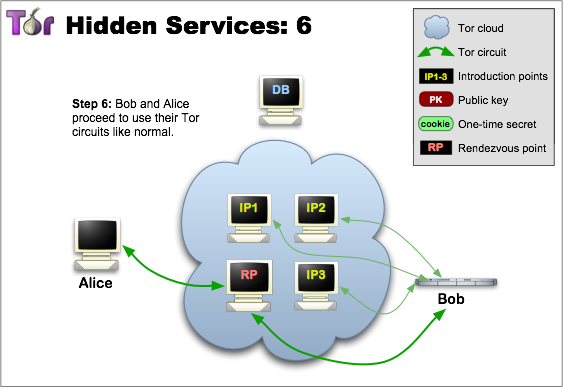
\includegraphics[width=0.5\textwidth]{THS-6}
    \caption{El punto de quedada notifica al cliente de que la conexión con el servicio oculto ha sido exitosa y ambos comienzan su comunicación de forma exitosa.}
    \label{ths6}
\end{figure}

\section{Ejemplo con Wireshark}

\bibliography{resumen.bib} %archivo citas.bib que contiene las entradas 
\bibliographystyle{siam} % haycle varias formas de citar

\end{document}